\documentclass{minimal}

\usepackage{tikz}

\usetikzlibrary{automata,positioning}

\begin{document}
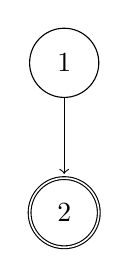
\begin{tikzpicture}[shorten >=1pt]
  \node[state] (1) {1};
  \node[state,accepting] (2) [below=of 1] {2};
  \path[->] (1) edge (2);
\end{tikzpicture}
%
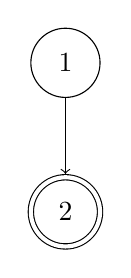
\begin{tikzpicture}[shorten >=1pt,accepting/.style={double distance=1.5pt}]
  \node[state] (1) {1};
  \node[state,accepting] (2) [below=of 1] {2};
  \path[->] (1) edge (2);
\end{tikzpicture}
%
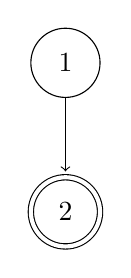
\begin{tikzpicture}[shorten >=1pt,accepting/.style={double distance=1.5pt}]
  \node[state] (1) {1};
  \node[state,accepting] (2) [below=of 1] {2};
  \path[->,shorten >=1.9pt] (1) edge (2);
\end{tikzpicture}
\end{document}